\documentclass[conference]{IEEEtran}
\IEEEoverridecommandlockouts
\usepackage{cite}
\usepackage{amsmath,amssymb,amsfonts}
\usepackage{graphicx}
\usepackage{booktabs}
\usepackage{multirow}
\usepackage{xcolor}
\usepackage{tikz}
\usetikzlibrary{positioning,arrows.meta,calc,shapes.geometric}
\usepackage[hidelinks]{hyperref}

\graphicspath{{figs/}}
\renewcommand{\topfraction}{0.9}
\renewcommand{\dbltopfraction}{0.9}
\renewcommand{\textfraction}{0.08}
\renewcommand{\floatpagefraction}{0.8}
\renewcommand{\dblfloatpagefraction}{0.8}
\setcounter{topnumber}{3}
\setcounter{dbltopnumber}{2}

\begin{document}

\title{Predicting Remaining Useful Life of Turbofan Engines from Raw Sensor History: Sequence Models and a Two-Stage Hybrid on NASA C-MAPSS FD001}

\author{\IEEEauthorblockN{Aryan, Akhil, Srijan, Abhayanth and Ashrith}
\IEEEauthorblockA{Deep Learning (DL) Course Project, Phase 2\\
Code and results: github.com/Abhayanthk/aml-rul-fd001}}

\maketitle

\begin{abstract}
We predict the Remaining Useful Life (RUL) of turbofan engines in the NASA C-MAPSS FD001 dataset. In Phase~1 we summarised the last 10 cycles of each sensor by hand and trained linear and tree models. The best of these, gradient boosting, had a validation RMSE of 40.17 cycles and a late-point RMSE (true RUL $\le 125$) of 26.54. Phase~2 asks whether models that read the \emph{raw} sensor history do better, and where.

We build leakage-free sensor windows and one shared training procedure. With these we compare five sequence architectures (LSTM, GRU, plain RNN, 1D CNN and CNN-LSTM), each trained once on the true RUL (\emph{uncapped}) and once on RUL capped at 125 (\emph{capped}). Every setting is chosen on a fixed validation set, and every model is averaged over five random seeds. A capped LSTM roughly halves the near-failure error (late RMSE 12.72 on validation, 13.36 on test). On its own, however, it fails our pre-registered cap rule, because it cannot predict long lives.

Our final model is a two-stage hybrid. The capped LSTM answers first; when it predicts more than 115 cycles, an uncapped LSTM takes over. On validation the hybrid has the lowest error of every single and two-stage model (RMSE 34.78\,$\pm$\,2.27, $R^2$ 0.67). On the test set, scored once, it beats every Phase~1 model (22.19 vs 25.33). The capped LSTM alone does even better on test (14.76), because the test set contains almost no engines far from failure. We report this disagreement instead of switching models after seeing the test set.
\end{abstract}

\begin{IEEEkeywords}
remaining useful life, predictive maintenance, C-MAPSS, LSTM, GRU, 1D CNN, RUL capping, two-stage model, early stopping
\end{IEEEkeywords}

\section{Introduction}
Aircraft engines wear out as they run. The Remaining Useful Life (RUL) of an engine is the number of operating cycles it has left before it fails. If an engine will fail at cycle 200 and we are at cycle 150, its RUL is 50. The model only sees the sensor readings up to the current cycle. A good RUL estimate lets maintenance be done just in time: too early wastes parts that still had life in them, and too late risks a failure.

\textbf{Phase 1 and its gap.} In Phase~1 we used the FD001 subset of NASA C-MAPSS \cite{saxena2008damage}. We built 57 features from 14 informative sensors: the current readings plus each sensor's mean, standard deviation and slope over the last 10 cycles. We then compared OLS, Elastic Net, Random Forest and gradient boosting. Gradient boosting was best, but the analysis showed two weaknesses:
\begin{itemize}
  \item close to failure the trees were still 26.5 cycles off on validation;
  \item far from failure every model struggled.
\end{itemize}
A 10-cycle summary cannot see a drift that builds up over tens of cycles.

\textbf{Phase 2 question.} \emph{Does a model that reads the raw sensor history beat the Phase~1 models built on hand-made features, and on which engines?} To answer this fairly we keep every Phase~1 rule: the same engine split, the same 100 validation points, the same test rows and the true RUL as the answer key.

\textbf{Contributions.}
\begin{enumerate}
  \item Leakage-free sensor windows and a single, frozen training procedure shared by every model (Sections~\ref{sec:data}--\ref{sec:models}).
  \item A controlled comparison of five sequence architectures, each uncapped and capped, with every setting chosen on validation and five seeds per final model (Section~\ref{sec:selection}).
  \item A two-stage hybrid that combines a near-failure expert with a long-life model. We compare it with a separate-classifier design and with ML\,+\,DL combinations (Section~\ref{sec:hybrid}).
  \item A single, one-time test evaluation of all 20 models, with an honest account of why validation and test disagree (Sections~\ref{sec:results}--\ref{sec:discussion}).
\end{enumerate}

\textbf{Team.} The work is one pipeline with five parts, each owned by one member, in this order:
\begin{enumerate}
  \item sequence windows (Aryan);
  \item training loop and uncapped LSTM (Akhil);
  \item capped LSTM, CNN and the RNN/GRU comparison (Srijan);
  \item cap rule and two-stage hybrid (Abhayanth);
  \item final comparison (Ashrith).
\end{enumerate}

\section{Related Work}
C-MAPSS \cite{saxena2008damage} simulates turbofan engines that run until they fail, and it is the standard benchmark for data-driven RUL estimation. Its FD001 subset has one operating condition and one fault mode. Recurrent networks with gated memory, the LSTM \cite{hochreiter1997lstm} and the GRU \cite{cho2014gru}, can keep information over long sequences. Zheng \emph{et al.} \cite{zheng2017lstm} showed that LSTMs beat feature-based regressors on C-MAPSS. Li \emph{et al.} \cite{li2018cnn} showed that 1D convolutions over time windows are also strong. Both lines of work train on a \emph{piecewise-linear} target that limits RUL to a constant early in life; our ``capped'' models use the same idea. Goel \emph{et al.} \cite{goel2026comparative} compare classical, CNN and LSTM models on C-MAPSS under a controlled recipe close to ours.

Muthukumar and Philip \cite{muthukumar2024cnnlstm} propose a CNN-LSTM hybrid. We test the idea but do not quote that paper's numbers, because its own results table is inconsistent: an MLP with RMSE 4.51 and $R^2$ 0.52 is listed next to a ``best'' CNN-LSTM with RMSE 13.34 and $R^2$ 0.86. Arunan \emph{et al.} \cite{arunan2024changepoint} first detect the health stage and then estimate RUL. Our two-stage hybrid follows the same idea, using the capped model's own prediction as the stage detector.

\section{Data and Evaluation Protocol}
\label{sec:data}

\subsection{Dataset and label}
FD001 has 100 training engines run until they fail (20{,}631 rows) and 100 test engines stopped some time before failure (13{,}096 rows). Each row is one engine at one cycle, with 3 operating settings and 21 sensors. We remove the 8 columns (one setting and 7 sensors) whose most common value fills $\ge 95\%$ of the training rows, which leaves 14 sensors. The label is RUL $=$ last cycle $-$ current cycle. It is never capped in the answer key.

\subsection{Splits}
The data is split \emph{by engine}, never by row: 80 training engines and 20 validation engines. Rows of one engine are near-copies of each other, so a row split would leak. The 20 validation engines contribute 100 fixed scoring points: five cut-off cycles per engine, drawn once with seed 42. Every model in both phases is scored on these same points. Of these, 22 are \emph{early} points (true RUL $>125$, up to 329) and 78 are \emph{late} points (true RUL $\le 125$).

The test set is the last row of each of the 100 test engines: 11 early and 89 late. Its largest true RUL is only 145. Test labels are loaded in exactly one notebook, after every model and setting has been fixed.

\subsection{Metrics}
The main metrics are MAE and RMSE in cycles. We also report:
\begin{itemize}
  \item $R^2$;
  \item early and late RMSE;
  \item late precision and recall, treating ``close to failure'' (prediction $\le 125$) as the positive class, so that low recall means dying engines called healthy;
  \item on test only, the NASA scoring function used in C-MAPSS papers \cite{saxena2008damage}.
\end{itemize}
The NASA score sums $e^{d/10}-1$ for $d>0$ and $e^{-d/13}-1$ for $d<0$, where $d=\hat y-y$. Predicting too much life is therefore punished much harder than predicting too little. We do not report the NASA score on validation: a few validation points with true RUL up to 329 push it into the millions for every model.

\subsection{Seeds and decision rules}
Neural network results depend on the random seed. Experiments use three seeds and every final model uses five (seeds 0--4). Each seed is scored on its own; we report the mean over seeds and the sample standard deviation of RMSE (written $\pm$). Predictions are never averaged across seeds before scoring.

Before seeing any result, we fixed a \emph{cap rule} in Phase~1 (21 October 2026): capped training is adopted only if, on validation, overall RMSE is no worse \emph{and} late RMSE is better.

\section{Sequence Windows (Aryan)}
A \emph{window} is the last $W$ cycles of one engine $\times$ the 14 sensors, a $W\times14$ matrix. Its label is the RUL at its last cycle (Fig.~\ref{fig:window}). Every training row gives one window that ends at that row. Four rules keep the windows free of leakage:
\begin{enumerate}
  \item \textbf{Scaling} uses each sensor's mean and standard deviation over the 80 training engines' rows only (e.g., \texttt{sensor\_2}: 642.6803 / 0.5028).
  \item \textbf{One engine:} a window never crosses two engines.
  \item \textbf{No future:} a window ends exactly at the cycle being predicted.
  \item \textbf{Padding:} an engine with fewer than $W$ cycles is padded by repeating its first (healthiest) row, which reads as ``no change yet''. Zero padding would be wrong, because after scaling 0 means an \emph{average} reading.
\end{enumerate}
Sixteen of the 80 training engines are held out for early stopping. They are drawn once with \texttt{default\_rng(0)}: engines 2, 3, 6, 16, 23, 26, 40, 44, 51, 57, 58, 67, 71, 75, 88 and 97. The remaining 64 \emph{fitting} engines give 13{,}118 training windows, and the held-out engines give 3{,}272 early-stopping windows.

At $W=30$ nothing needs padding, since the shortest test engine has 31 cycles. At $W=70$, 20 validation points and 14 test engines are padded. Automated checks confirm all four rules, for example by replacing sensor values with the engine id and the cycle number and building the windows the same way.

\begin{figure}[t]
\centering
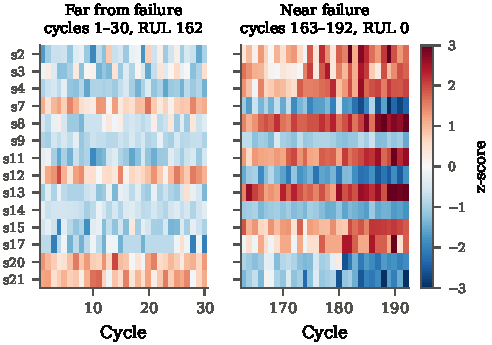
\includegraphics[width=\columnwidth]{window.pdf}
\caption{One training engine seen through two 30-cycle windows. Far from failure the sensors are noise around their means; near failure several sensors drift strongly (red: above the training mean, blue: below).}
\label{fig:window}
\end{figure}

\section{Models and Training (Akhil, Srijan)}
\label{sec:models}

\subsection{Architectures}
All models read a $W\times14$ window. The recurrent models end in the same head: last-cycle output $\to$ dropout 0.2 $\to$ dense 32 + ReLU $\to$ dense 1. Table~\ref{tab:models} lists the models and their sizes.

\textbf{LSTM.} At each cycle the LSTM \cite{hochreiter1997lstm} updates a memory cell $c_t$ through three gates:
\begin{align}
f_t,i_t,o_t &= \sigma\big(W_{\{f,i,o\}}[h_{t-1},x_t]+b_{\{f,i,o\}}\big),\\
c_t &= f_t\odot c_{t-1}+i_t\odot\tanh(W_c[h_{t-1},x_t]+b_c),\\
h_t &= o_t\odot\tanh(c_t).
\end{align}
The forget gate $f_t$ drops old memory, the input gate $i_t$ adds new information, and the output gate $o_t$ decides what to pass on. The additive update of $c_t$ lets a slow drift build up over 30--70 cycles, which a 10-cycle summary cannot capture.

\textbf{Comparison models.}
\begin{itemize}
  \item The \textbf{GRU} \cite{cho2014gru} has two gates and no separate memory cell.
  \item The plain \textbf{RNN} has no gates and serves as a control that shows what gating adds.
  \item The \textbf{1D CNN} has three convolutions sliding over \emph{time only}: 32, 64 and 64 filters with kernel sizes 5, 5 and 3, ReLU, and dropout 0.3. They are followed by flatten $\to$ dense 128 $\to$ dense 1. Flattening keeps \emph{when} a pattern happened; an earlier version with global average pooling lost that information and was the weakest model.
  \item The \textbf{CNN-LSTM} \cite{muthukumar2024cnnlstm} adds one convolution (64 filters, kernel 5) and max pooling before a $2\times64$ LSTM.
\end{itemize}

\begin{table}[t]
\centering
\caption{Models and trainable weights (uncapped / capped)}
\label{tab:models}
\setlength{\tabcolsep}{4pt}
\begin{tabular}{@{}lll@{}}
\toprule
Model & Size (uncapped / capped) & Weights \\
\midrule
LSTM & $2\times64$ / $1\times64$ & 55{,}873 / 22{,}593 \\
GRU & $2\times64$ / $1\times64$ & 42{,}433 / 17{,}473 \\
RNN & $2\times64$ / $1\times64$ & 15{,}553 / 7{,}233 \\
1D CNN & 3 conv + 2 dense & 270{,}945 / 598{,}625 \\
CNN-LSTM & 1 conv + pool + $2\times64$ & 73{,}217 \\
\bottomrule
\end{tabular}
\end{table}

\subsection{Shared training procedure}
Every model is trained with the same frozen procedure, implemented once in \texttt{train.py}:
\begin{itemize}
  \item \textbf{Target and loss:} RUL$/100$ (capped: $\min(\mathrm{RUL},125)/100$), mean squared error.
  \item \textbf{Optimiser:} Adam \cite{kingma2015adam}, learning rate 0.001 (0.003 for the capped models, except the 1D CNN), no weight decay.
  \item \textbf{Batches:} size 128, reshuffled every epoch.
  \item \textbf{Stability:} gradient clipping at norm 1.0 \cite{pascanu2013difficulty}; the learning rate halves after 5 epochs without improvement.
  \item \textbf{Early stopping:} training stops after 15 epochs without improvement on the 16 held-out engines, at most 150 epochs, and the best weights are restored.
  \item \textbf{Seeding:} the seed is set before the model is built.
\end{itemize}
Uncapped models read $W=30$ cycles and capped models read $W=70$. All training ran on CPU with PyTorch \cite{paszke2019pytorch}; a run takes 6--200\,s.

Early stopping matters because the best epoch varies widely. In the run in Fig.~\ref{fig:curve}, the held-out loss is best at epoch 3 while the fitting loss keeps falling. Across runs, training stopped after 16 to 77 epochs.

\begin{figure}[t]
\centering
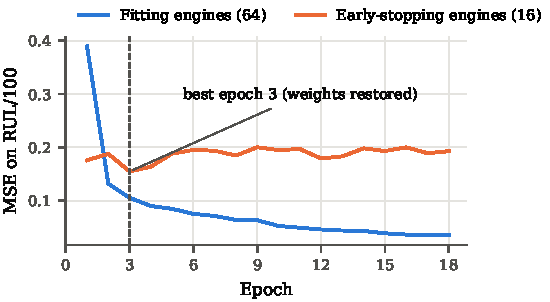
\includegraphics[width=\columnwidth]{curve.pdf}
\caption{Uncapped LSTM ($W=30$, $2\times64$, seed 0). The held-out loss bottoms out early while the fitting loss keeps falling; early stopping restores the best epoch.}
\label{fig:curve}
\end{figure}

\subsection{Capped vs uncapped training}
An \emph{uncapped} model learns the true RUL, so it can predict 200 or 300. A \emph{capped} model learns $\min(\mathrm{RUL},125)$. It treats every engine with more than 125 cycles left as ``healthy = 125'' and spends its capacity on the part of life where the sensors actually change (Fig.~\ref{fig:sensor4}). Scoring always uses the true RUL, so a capped model's misses on long-lived engines are fully counted.

\begin{figure}[t]
\centering
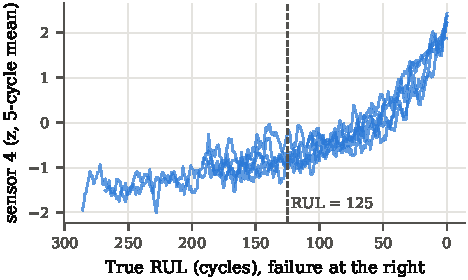
\includegraphics[width=\columnwidth]{sensor4.pdf}
\caption{Scaled \texttt{sensor\_4} against true RUL for five training engines. The sensor is flat noise until about 125 cycles before failure, then rises. An engine with 250 cycles left looks like one with 150 left.}
\label{fig:sensor4}
\end{figure}

\section{Model Selection on Validation}
\label{sec:selection}

\begin{table*}[t]
\centering
\caption{All models on validation (100 points: 22 early, 78 late) and test (100 engines: 11 early, 89 late). Phase~1 rows are single runs; Phase~2 rows are the mean of 5 seeds, $\pm$ is the sample std of RMSE. Early/late RMSE split at true RUL 125. Recall: share of late points predicted $\le125$. NASA score on test only (lower is better).}
\label{tab:final}
\scriptsize
\setlength{\tabcolsep}{3.2pt}
\begin{tabular}{@{}l cccccc ccccc r@{}}
\toprule
 & \multicolumn{6}{c}{Validation} & \multicolumn{6}{c}{Test (scored once)} \\
\cmidrule(lr){2-7}\cmidrule(l){8-13}
Model & MAE & RMSE & $R^2$ & Early & Late & Recall & MAE & RMSE & $R^2$ & Early & Late & NASA \\
\midrule
\multicolumn{13}{@{}l}{\emph{Phase 1 (engineered features)}}\\
OLS & 32.86 & 42.92 & 0.50 & 64.87 & 34.27 & 0.76 & 24.91 & 31.17 & 0.44 & 23.00 & 32.04 & 11,407\\
Elastic Net & 31.66 & 41.77 & 0.53 & 66.02 & 31.74 & 0.79 & 23.61 & 29.04 & 0.51 & 20.60 & 29.92 & 5,620\\
Random Forest & 25.03 & 40.17 & 0.56 & 69.59 & 26.50 & 0.86 & 18.95 & 25.88 & 0.61 & 25.80 & 25.89 & 6,048\\
Gradient boosting & 26.12 & 40.17 & 0.56 & 69.54 & 26.54 & 0.86 & 18.54 & 25.33 & 0.63 & 22.98 & 25.61 & 4,813\\
\midrule
\multicolumn{13}{@{}l}{\emph{Phase 2, uncapped ($W{=}30$)}}\\
LSTM & 23.48 & 36.28\,$\pm$\,3.14 & 0.64 & 62.96 & 23.78 & 0.86 & 19.70 & 28.52\,$\pm$\,2.66 & 0.53 & 33.78 & 27.62 & 32,544\\
GRU & 22.82 & 35.76\,$\pm$\,0.53 & 0.65 & 62.57 & 23.07 & 0.88 & 18.47 & 26.99\,$\pm$\,2.69 & 0.57 & 21.68 & 27.55 & 16,470\\
RNN & 27.05 & 39.40\,$\pm$\,2.68 & 0.58 & 62.16 & 29.72 & 0.82 & 23.94 & 32.71\,$\pm$\,2.62 & 0.38 & 22.88 & 33.67 & 54,422\\
1D CNN & 25.43 & 40.14\,$\pm$\,1.69 & 0.56 & 72.75 & 23.78 & 0.93 & 18.13 & 24.21\,$\pm$\,2.58 & 0.66 & 17.34 & 24.92 & 4,996\\
CNN-LSTM & 24.02 & 37.33\,$\pm$\,1.11 & 0.62 & 64.52 & 24.62 & 0.87 & 18.86 & 25.94\,$\pm$\,3.35 & 0.61 & 21.66 & 26.35 & 9,550\\
\midrule
\multicolumn{13}{@{}l}{\emph{Phase 2, capped ($W{=}70$)}}\\
LSTM & 21.25 & 39.79\,$\pm$\,0.59 & 0.57 & 81.35 & 12.72 & 1.00 & 11.13 & 14.76\,$\pm$\,0.26 & 0.87 & 23.14 & 13.36 & 343\\
GRU & 21.25 & 39.38\,$\pm$\,0.68 & 0.58 & 79.95 & 13.55 & 0.99 & 11.25 & 14.93\,$\pm$\,1.08 & 0.87 & 22.00 & 13.78 & 354\\
RNN & 24.43 & 41.96\,$\pm$\,0.69 & 0.52 & 82.56 & 18.29 & 0.99 & 13.33 & 17.99\,$\pm$\,1.41 & 0.81 & 23.66 & 17.14 & 903\\
1D CNN & 23.66 & 42.03\,$\pm$\,1.13 & 0.52 & 84.99 & 15.02 & 0.99 & 13.13 & 16.83\,$\pm$\,0.86 & 0.84 & 26.24 & 15.20 & 490\\
CNN-LSTM & 21.32 & 39.76\,$\pm$\,1.27 & 0.57 & 80.55 & 13.95 & 0.99 & 11.97 & 15.74\,$\pm$\,1.01 & 0.86 & 21.70 & 14.77 & 424\\
\midrule
\multicolumn{13}{@{}l}{\emph{Phase 2, two-stage and blends}}\\
\textbf{Two-stage hybrid (final)} & 20.32 & 34.78\,$\pm$\,2.27 & 0.67 & 68.40 & 15.15 & 0.95 & 14.70 & 22.19\,$\pm$\,1.74 & 0.71 & 30.46 & 20.84 & 16,337\\
Capped LSTM + GB fallback & 19.91 & 35.22\,$\pm$\,1.28 & 0.66 & 69.84 & 14.61 & 0.96 & 14.08 & 20.14\,$\pm$\,0.76 & 0.76 & 23.48 & 19.68 & 3,030\\
Classifier + late regressor & 23.22 & 40.33\,$\pm$\,1.24 & 0.56 & 78.83 & 18.17 & 1.00 & 12.71 & 18.19\,$\pm$\,0.92 & 0.81 & 23.33 & 17.37 & 1,195\\
0.2 GB + 0.8 LSTM uncapped & 23.53 & 35.98\,$\pm$\,2.43 & 0.65 & 63.43 & 22.85 & 0.87 & 18.48 & 26.24\,$\pm$\,2.13 & 0.60 & 28.20 & 25.87 & 12,735\\
0.1 GB + 0.9 hybrid & 20.34 & 34.71\,$\pm$\,1.95 & 0.67 & 68.03 & 15.39 & 0.95 & 14.51 & 21.74\,$\pm$\,1.53 & 0.73 & 28.74 & 20.64 & 10,011\\
0.5 GB + 0.5 LSTM capped & 22.44 & 38.29\,$\pm$\,0.37 & 0.60 & 74.32 & 17.93 & 0.91 & 13.12 & 17.76\,$\pm$\,0.18 & 0.82 & 18.38 & 17.68 & 786\\
\bottomrule

\end{tabular}
\end{table*}

All choices in this section use validation only.

\subsection{Uncapped LSTM: window and size (Akhil)}
Table~\ref{tab:uncapped} shows the uncapped grid (3 seeds). A 30-cycle window beats 50 and 70: far from failure, extra history adds flat readings, not signal. With two layers of 64 units the error was lowest and most stable. The 32-unit models were unstable, and the 128-unit models were no better but 1.4--3.7$\times$ slower; $2\times128$ has about 210k weights for 64 fitting engines.

\begin{table}[t]
\centering
\caption{Uncapped LSTM selection (validation, 3 seeds)}
\label{tab:uncapped}
\setlength{\tabcolsep}{4pt}
\begin{tabular}{@{}llcc@{}}
\toprule
Grid & Setting & RMSE & Late RMSE \\
\midrule
\multirow{3}{*}{\shortstack[l]{Window\\(1$\times$64)}} & $W=30$ & \textbf{36.59 $\pm$ 2.17} & \textbf{21.84} \\
 & $W=50$ & 38.63 $\pm$ 2.32 & 25.68 \\
 & $W=70$ & 38.69 $\pm$ 4.74 & 25.14 \\
\midrule
\multirow{6}{*}{\shortstack[l]{Size\\($W=30$)}} & 32$\times$1 & 37.69 $\pm$ 4.23 & 26.01 \\
 & 32$\times$2 & 39.36 $\pm$ 5.00 & 29.43 \\
 & 64$\times$1 & 36.59 $\pm$ 2.17 & 21.84 \\
 & \textbf{64$\times$2} & \textbf{34.28 $\pm$ 0.94} & 23.56 \\
 & 128$\times$1 & 38.34 $\pm$ 3.56 & 24.85 \\
 & 128$\times$2 & 35.34 $\pm$ 6.07 & 27.23 \\
\bottomrule
\end{tabular}
\end{table}

\subsection{Capped LSTM: window (Srijan)}
For the capped model, late RMSE is what matters. A longer history helps near failure (3 seeds, $1\times64$, lr 0.001): late RMSE falls from 15.69 ($W=30$) to 13.95 ($W=50$) and 12.23 ($W=70$), while overall RMSE stays near 40. Near failure, the \emph{shape} of the decline over 70 cycles is informative. We chose $W=70$, $1\times64$ and lr 0.003; larger models added no accuracy.

\subsection{Memory ladder and CNNs (Srijan, Akhil)}
Table~\ref{tab:ladder} compares architectures with the chosen LSTM settings, so that only the network changes (5 seeds).
\begin{itemize}
  \item \textbf{Gates help.} The RNN is the worst recurrent model in both settings, because early information fades over 30--70 steps.
  \item \textbf{GRU vs LSTM.} On the uncapped job the GRU ties the LSTM (35.76 vs 36.28, inside the seed spread) and is steadier. With three seeds the order was reversed (LSTM 34.28 vs GRU 35.97), which is why final comparisons use five. Near failure the LSTM is better (late 12.72 vs 13.55). That is the job the hybrid relies on most, so the LSTM stays.
  \item \textbf{CNN.} The 1D CNN loses in both settings, with 5--26$\times$ more weights, almost all in the flatten $\to$ dense layer.
  \item \textbf{CNN-LSTM.} It comes close to the capped LSTM but does not beat it.
\end{itemize}

\begin{table}[t]
\centering
\caption{Architecture comparison (validation, 5 seeds)}
\label{tab:ladder}
\setlength{\tabcolsep}{4pt}
\begin{tabular}{@{}lcccc@{}}
\toprule
 & \multicolumn{2}{c}{Uncapped ($W=30$)} & \multicolumn{2}{c}{Capped ($W=70$)} \\
\cmidrule(lr){2-3}\cmidrule(lr){4-5}
Model & RMSE & Late & RMSE & Late \\
\midrule
RNN & 39.40 $\pm$ 2.68 & 29.72 & 41.96 $\pm$ 0.69 & 18.29 \\
GRU & \textbf{35.76 $\pm$ 0.53} & \textbf{23.07} & \textbf{39.38 $\pm$ 0.68} & 13.55 \\
LSTM & 36.28 $\pm$ 3.14 & 23.78 & 39.79 $\pm$ 0.59 & \textbf{12.72} \\
1D CNN & 40.14 $\pm$ 1.69 & 23.78 & 42.03 $\pm$ 1.13 & 15.02 \\
CNN-LSTM & 37.33 $\pm$ 1.11 & 24.62 & 39.76 $\pm$ 1.27 & 13.95 \\
\bottomrule
\end{tabular}
\end{table}

\section{Cap Rule and Two-Stage Hybrid (Abhayanth)}
\label{sec:hybrid}

\begin{figure*}[t]
\centering
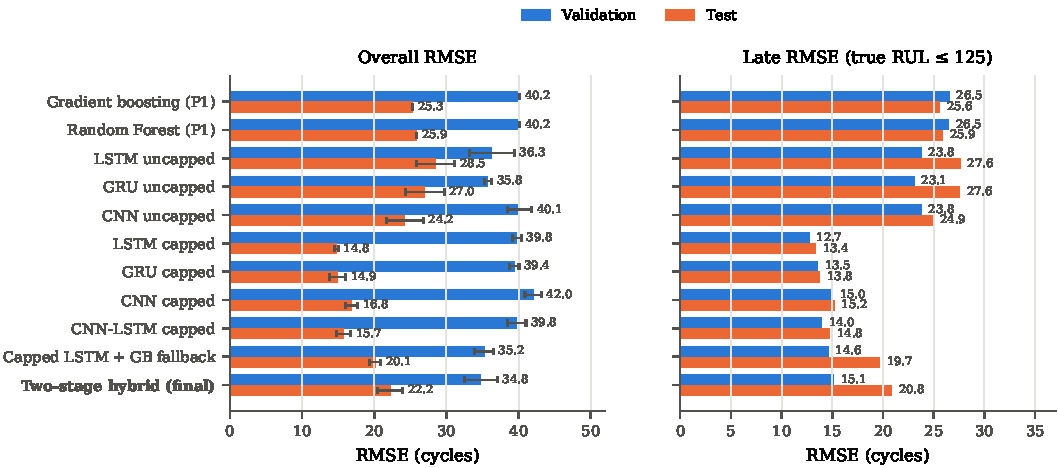
\includegraphics[width=\textwidth]{rmse_bars.pdf}
\caption{Overall RMSE (left, error bars: std over 5 seeds) and late RMSE (right) on validation and test for the main models. Every capped model, and every design built on the capped LSTM, cuts Phase~1's error near failure; the capped LSTM roughly halves it.}
\label{fig:bars}
\end{figure*}

\begin{figure*}[t]
\centering
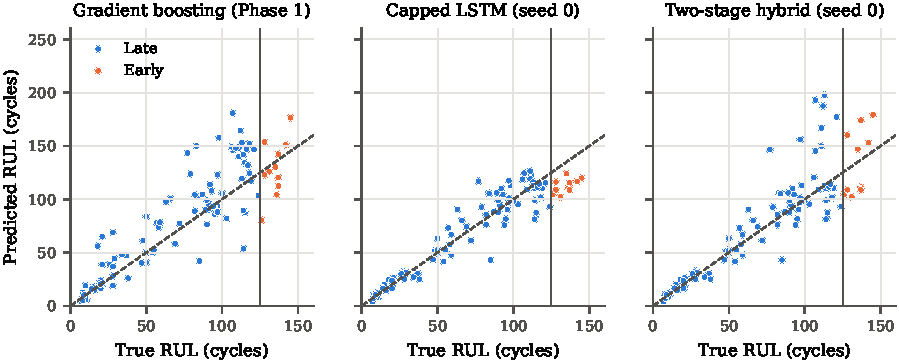
\includegraphics[width=0.92\textwidth]{pred_vs_true_test.pdf}
\caption{Predicted vs true RUL on the test set (seed 0 for the LSTMs). Points above the dashed diagonal predict too much life, the dangerous side. The vertical line marks true RUL $=125$.}
\label{fig:pred}
\end{figure*}





\subsection{Capping alone fails the cap rule}
The capped LSTM cuts late RMSE from 23.78 to 12.72, but its overall RMSE is worse (39.79 vs 36.28), because it never predicts much above 125 for healthy engines (early RMSE 81.35). Both conditions of the cap rule are required, so the rule returns \textbf{FAIL}: capping cannot be the whole answer.

\subsection{The two-stage hybrid}
The two LSTMs are good at opposite jobs, so we combine them (Fig.~\ref{fig:hybrid}). The capped LSTM ($W=70$) predicts $p$. If $p\le115$, the answer is $p$. Otherwise the engine looks healthy and the uncapped LSTM ($W=30$) predicts $q$; the answer is $\max(q,p)$. A lower $q$ would contradict the gate, which has already judged the engine healthy. Capped seed $s$ is paired with uncapped seed $s$, each pair is scored, and the five pairs are averaged.

\begin{figure}[t]
\centering
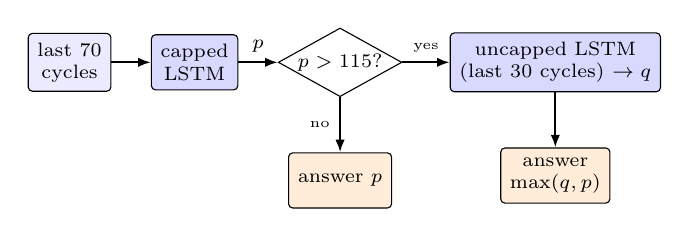
\begin{tikzpicture}[
  node distance=4mm and 5mm,
  box/.style={draw, rounded corners=1.5pt, minimum height=7mm, align=center, font=\scriptsize, fill=#1},
  box/.default=white,
  arr/.style={-{Latex[length=1.6mm]}, thick}]
\node[box=blue!8] (w70) {last 70\\cycles};
\node[box=blue!15, right=of w70] (cap) {capped\\LSTM};
\node[draw, diamond, aspect=1.8, inner sep=0.5pt, font=\scriptsize, right=of cap] (gate) {$p>115$?};
\node[box=orange!15, below=7mm of gate] (ans1) {answer $p$};
\node[box=blue!15, right=6mm of gate] (unc) {uncapped LSTM\\(last 30 cycles) $\to q$};
\node[box=orange!15, below=7mm of unc] (ans2) {answer\\$\max(q,p)$};
\draw[arr] (w70) -- (cap);
\draw[arr] (cap) -- node[above, font=\scriptsize]{$p$} (gate);
\draw[arr] (gate) -- node[left, font=\tiny]{no} (ans1);
\draw[arr] (gate) -- node[above, font=\tiny]{yes} (unc);
\draw[arr] (unc) -- (ans2);
\end{tikzpicture}
\caption{The final two-stage hybrid. The capped LSTM is the near-failure expert and also acts as the gate.}
\label{fig:hybrid}
\end{figure}

\textbf{Gate threshold.} Table~\ref{tab:gate} tries gates of 100--120. A \emph{missed late} point is a near-failure engine that the gate hands to the uncapped model as if it were healthy, which is the dangerous error.
\begin{itemize}
  \item \textbf{Gates 100 and 110} give a slightly lower RMSE but miss 9--21 late points per seed.
  \item \textbf{Gate 120} barely fires, so the hybrid collapses to the capped model.
  \item \textbf{Gate 115 (chosen)} misses 4.6 points per seed, all with true RUL 89--121, close to the 125 line.
\end{itemize}
A gate of 125 would never fire, because the capped model almost never predicts above about 123.

\begin{table}[t]
\centering
\caption{Gate threshold (validation, 5 seed pairs)}
\label{tab:gate}
\setlength{\tabcolsep}{4pt}
\begin{tabular}{@{}ccccc@{}}
\toprule
Gate & Sent to uncapped & Missed late (RUL) & RMSE & Late RMSE \\
\midrule
100 & 41.4 & 20.6 (66--121) & 33.37 $\pm$ 2.65 & 17.70 \\
110 & 26.8 & 9.2 (84--121) & 33.45 $\pm$ 2.52 & 16.35 \\
\textbf{115} & 17.2 & \textbf{4.6} (89--121) & 34.78 $\pm$ 2.27 & 15.15 \\
120 & 6.0 & 1.8 (108--121) & 39.23 $\pm$ 0.59 & 13.98 \\
\bottomrule
\end{tabular}
\end{table}

\subsection{Rejected and alternative designs}
\textbf{Separate classifier.} We replaced the gate with a dedicated LSTM classifier trained on ``true RUL $>125$''. Engines it labels late went to a regressor trained only on late rows. Over 3 seeds the classifier was 77\% accurate, but it called 17 of 78 near-failure points healthy, and late RMSE rose to 18.36. A yes/no decision at 125 is harder to learn than a number, and the capped model's own output already carries that information.

\textbf{ML\,+\,DL combinations.} Using Phase~1 gradient boosting (GB) as the fallback for healthy engines, with the same gate, ties the hybrid on validation: 35.22\,$\pm$\,1.28 vs 34.78\,$\pm$\,2.27. It is steadier, because GB gives the same answer every run. We report it alongside the hybrid but did not choose it: it only ties, and the LSTM hybrid had been chosen first. Weighted averages of GB with a deep model, with the weight chosen on validation, move RMSE by 0.3 or less. A 50/50 blend with the capped LSTM worsens late RMSE from 12.72 to 17.93.

\section{Final Results (Ashrith)}
\label{sec:results}


\begin{figure}[t]
\centering
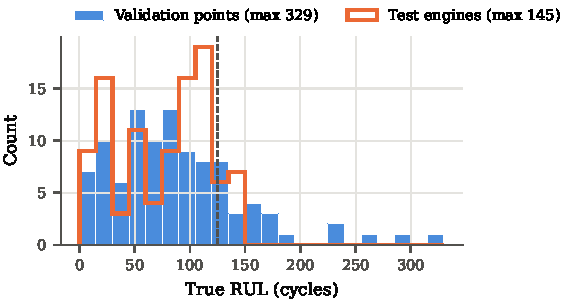
\includegraphics[width=\columnwidth]{val_vs_test.pdf}
\caption{True RUL at the 100 validation points and the 100 test engines. The dashed line marks 125. Test has few long-lived engines.}
\label{fig:valtest}
\end{figure}

Table~\ref{tab:final} scores all 20 models on validation and, once, on test. Fig.~\ref{fig:bars} shows overall and late RMSE for the main models.



\textbf{Overall winner on validation.} The two-stage hybrid has the lowest RMSE of every single and two-stage model (34.78\,$\pm$\,2.27, MAE 20.32, $R^2$ 0.67), compared with 40.17 and $R^2$ 0.56 for gradient boosting. Only a blend that adds 10\% gradient boosting to the hybrid is marginally lower (34.71), a difference far inside the seed spread. Its late RMSE (15.15) is close to the capped expert's and far below Phase~1's 26.54. It is the only design that is both no worse overall and much better late, so it passes the spirit of the cap rule.

\textbf{Near-failure error is roughly halved.} Late RMSE falls from 26.54 (GB) to 12.72 (capped LSTM) on validation and from 25.61 to 13.36 on test. Every capped model lies between 12.72 and 18.29 on validation.

\textbf{Test.} The hybrid beats every Phase~1 model on test (RMSE 22.19 vs 25.33). Several capped single models do better still: the capped LSTM reaches 14.76\,$\pm$\,0.26 with $R^2$ 0.87, which is 42\% below gradient boosting and close to published FD001 LSTM results of about 15--16. Fig.~\ref{fig:pred} shows why: the capped LSTM stays close to the diagonal on the test engines, while the hybrid hands some late engines to the uncapped model, which over-predicts them.


\section{Discussion}
\label{sec:discussion}

\subsection{Why validation and test disagree}
Validation and test contain different kinds of engines (Fig.~\ref{fig:valtest}). Validation has 22 far-from-failure points with true RUL up to 329. Test has only 11, and its largest true RUL is 145. A capped model cannot miss badly when nothing is far from failure, so this test set favours capping. The hybrid exists to handle long-lived engines, and this test set barely contains any.

We chose the hybrid on validation before scoring test. Switching to the capped LSTM after seeing the test numbers would make the test score meaningless as an estimate of performance on unseen engines. The correct reading is that the best model depends on the engines being monitored. If engines can be far from failure, use the hybrid. If they are known to be close to failure, the capped LSTM alone is better.


\subsection{Known weaknesses of the hybrid}
\textbf{The gate is less reliable on test.} Late engines handed to the uncapped model, per seed:
\begin{itemize}
  \item validation: 5, 4, 6, 3 and 5 (true RUL 89--121);
  \item test: 10, 8, 9, 14 and 13 (true RUL 77--121; 44 of 54 above 100).
\end{itemize}
This is why the hybrid's test late RMSE (20.84) is higher than the capped LSTM's (13.36).

\textbf{The NASA score punishes over-prediction.} When the uncapped LSTM over-predicts, the exponential penalty dominates. Over-predictions account for 95.5--99.8\% of the hybrid's NASA score, which ranges from 2{,}754 to 45{,}410 across seeds (mean 16{,}337). In one seed, a single engine with 137 cycles left was predicted at 241, which alone adds 33{,}606. The GB-fallback version over-predicts far less (3{,}030), and the capped LSTM scores 343.

\subsection{Far-from-failure engines and seeds}
Early RMSE on validation is 62--85 for every model in both phases. A healthy engine's sensors have not started to drift (Fig.~\ref{fig:sensor4}), so 200 and 300 cycles left look the same. This is a limit of the data, not of the models. It is also why uncapped models vary so much between seeds: for the uncapped LSTM, RMSE ranges from 33.2 to 41.2 across seeds, almost entirely because of the early points. With three seeds the LSTM and GRU ranked the other way round; one seed can crown a lucky model.

\subsection{Reading the classification metrics}
Capped models reach late recall of 0.99--1.00 on validation simply because they almost never predict above 125. Their precision (0.78--0.80) shows the cost: healthy engines sent to maintenance early. Recall should therefore never be read alone. $R^2$ ranks models in the same order as RMSE within a set, but it is easier to interpret: the hybrid explains 67\% of the variation on validation, and gradient boosting 56\%.

\subsection{Limitations}
\begin{itemize}
  \item Only FD001 was used: one operating condition and one fault mode.
  \item Validation contains just 22 early points and test just 11, so early RMSE is noisy.
  \item Settings were tuned for the LSTM; a GRU-specific search could close the remaining near-failure gap.
  \item The hybrid's gate threshold and the GB blend weights were chosen on the same 100 validation points as the architectures.
\end{itemize}

\section{Conclusion}
Reading the raw sensor history helps exactly where it matters most, close to failure. A capped LSTM roughly halves the near-failure error of the best Phase~1 model on both validation and test. Capping alone fails our pre-registered cap rule, because it cannot predict long lives. A two-stage hybrid, in which the capped LSTM acts as both the near-failure expert and the gate for an uncapped LSTM, has the lowest validation error of every single and two-stage model (RMSE 34.78, $R^2$ 0.67) and beats every Phase~1 model on test.

Among the architectures:
\begin{itemize}
  \item gated recurrent models clearly beat a plain RNN;
  \item the GRU ties the LSTM far from failure, but the LSTM is better near failure;
  \item 1D CNNs and CNN-LSTMs add weights without adding accuracy on 64 fitting engines.
\end{itemize}

Engines far from failure remain hard for every model. The validation--test disagreement shows that the right model depends on how far from failure the monitored engines are. Next steps are the other C-MAPSS subsets (FD002--FD004, with several operating conditions and fault modes) and an interval output such as ``more than 115 cycles left'' for engines the gate judges healthy.

\section*{Author Contributions}
\begin{itemize}
  \item \textbf{Aryan:} sequence windows, scaling, early-stopping engines and leakage checks (\texttt{sequences.py}, notebook 06).
  \item \textbf{Akhil:} shared training procedure, LSTM and CNN-LSTM models, uncapped LSTM selection (\texttt{train.py}, \texttt{models\_lstm.py}, notebook 07).
  \item \textbf{Srijan:} capped LSTM, 1D CNN and the RNN/GRU comparison (\texttt{models\_cnn.py}, \texttt{models\_rnn\_gru.py}, notebook 08).
  \item \textbf{Abhayanth:} cap rule, two-stage hybrid, classifier and ML\,+\,DL alternatives, decision log (notebook 09).
  \item \textbf{Ashrith:} final comparison on validation and test (notebook 10).
\end{itemize}
Every number in this report comes from the files in \texttt{results/} of the project repository.

\bibliographystyle{IEEEtran}
\begin{thebibliography}{11}

\bibitem{saxena2008damage}
A.~Saxena, K.~Goebel, D.~Simon, and N.~Eklund, ``Damage propagation modeling for aircraft engine run-to-failure simulation,'' in \emph{Proc. Int. Conf. Prognostics and Health Management (PHM)}, Denver, CO, USA, 2008, pp. 1--9.

\bibitem{hochreiter1997lstm}
S.~Hochreiter and J.~Schmidhuber, ``Long short-term memory,'' \emph{Neural Computation}, vol.~9, no.~8, pp. 1735--1780, 1997.

\bibitem{cho2014gru}
K.~Cho, B.~van Merri\"enboer, C.~Gulcehre, D.~Bahdanau, F.~Bougares, H.~Schwenk, and Y.~Bengio, ``Learning phrase representations using RNN encoder-decoder for statistical machine translation,'' in \emph{Proc. Conf. Empirical Methods in Natural Language Processing (EMNLP)}, 2014, pp. 1724--1734.

\bibitem{zheng2017lstm}
S.~Zheng, K.~Ristovski, A.~Farahat, and C.~Gupta, ``Long short-term memory network for remaining useful life estimation,'' in \emph{Proc. IEEE Int. Conf. Prognostics and Health Management (ICPHM)}, 2017, pp. 88--95.

\bibitem{li2018cnn}
X.~Li, Q.~Ding, and J.-Q. Sun, ``Remaining useful life estimation in prognostics using deep convolution neural networks,'' \emph{Reliability Engineering \& System Safety}, vol.~172, pp. 1--11, 2018.

\bibitem{goel2026comparative}
A.~Goel, S.~Galchar, and S.~Kanu, ``Remaining useful life estimation for turbofan engines: A comparative study of classical, CNN, and LSTM approaches,'' arXiv:2604.27234, 2026.

\bibitem{muthukumar2024cnnlstm}
G.~Muthukumar and J.~Philip, ``CNN-LSTM hybrid deep learning model for remaining useful life estimation,'' arXiv:2412.15998, 2024.

\bibitem{arunan2024changepoint}
A.~Arunan, Y.~Qin, X.~Li, and C.~Yuen, ``A change point detection integrated remaining useful life estimation model under variable operating conditions,'' \emph{Control Engineering Practice}, 2024, arXiv:2401.04351.

\bibitem{kingma2015adam}
D.~P. Kingma and J.~Ba, ``Adam: A method for stochastic optimization,'' in \emph{Proc. Int. Conf. Learning Representations (ICLR)}, 2015.

\bibitem{pascanu2013difficulty}
R.~Pascanu, T.~Mikolov, and Y.~Bengio, ``On the difficulty of training recurrent neural networks,'' in \emph{Proc. Int. Conf. Machine Learning (ICML)}, 2013, pp. 1310--1318.

\bibitem{paszke2019pytorch}
A.~Paszke \emph{et al.}, ``PyTorch: An imperative style, high-performance deep learning library,'' in \emph{Advances in Neural Information Processing Systems (NeurIPS)}, vol.~32, 2019.

\end{thebibliography}

\end{document}
